\documentclass{beamer}
\usetheme{EMBL}
\usepackage{tikz}
\usepackage{lpc}

\title[Jug]{Jug: Executing Parallel Tasks in Python}
\author{Luis Pedro Coelho}
\institute{EMLB}
\date{21 May 2013}

\def\iverson#1{%
\ensuremath{[}#1\ensuremath{]}%
}

\graphicspath{{figures/}{figures/generated/}{images/}}

\begin{document}
\frame{\titlepage}

\begin{frame}[fragile]
\frametitle{Jug: Coarse Parallel Tasks in Python}

\begin{itemize}
\item Parallel Python code
\item Memoization
\end{itemize}
\end{frame}

\begin{frame}[fragile]
\frametitle{Parallel Problem (Example)}

\begin{block}{Members of Parliament}
Given a list of the Wikipedia page for all British MPs.
\begin{itemize}
\item Get word counts for each page
\item Merge the word counts
\item Get over-represented counts for each MP
\end{itemize}
\end{block}

\end{frame}

\begin{frame}[fragile]
\frametitle{Fan-Out/Fan-In Dependency Structure}

\begin{center}
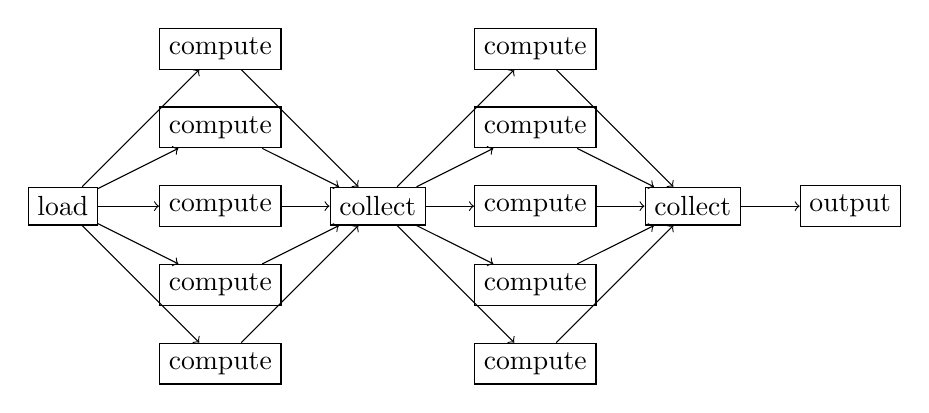
\begin{tikzpicture}
\node (load) at (0,0) [draw] {load};
\node (collect) at (4,0) [draw] {collect};
\node (collect2) at (8,0) [draw] {collect};
\node (output) at (10,0) [draw] {output};

\path[->]
    (collect2) edge (output);

\foreach \y in {-2,-1,0,1,2} {%
    \node (compute\y) at (2,\y) [draw] {compute};
    \path[->]
        (load) edge (compute\y)
        (compute\y) edge (collect);
}

\foreach \y in {-2,-1,0,1,2} {%
    \node (compute2\y) at (6,\y) [draw] {compute};
    \path[->]
        (collect) edge (compute2\y)
        (compute2\y) edge (collect2);
}
\end{tikzpicture}

\end{center}

\end{frame}

\begin{frame}[fragile]
\frametitle{Jug Processes are Separate Processes!}
\begin{itemize}
\item \alert{No Global Interpreter Lock} issues
\item Can run on \alert{separate machines}
\item Do not need to start at the same time
\end{itemize}
\end{frame}

\begin{frame}[fragile]
\frametitle{Two Backends Are Available}
\begin{block}{Filesystem}
\begin{itemize}
\item Default backend
\item Carefully designed to work on NFS
\item Anything pickle()able can be used as Task output/input.
\item Numpy arrays are special-cased (for speed and disk-space savings).
\end{itemize}
\end{block}

\begin{block}{Redis (NoSQL Database)}
\begin{itemize}
\item Redis is a file-backed store
\item Ideal for many small ``files''
\item All workers talk to same database
\end{itemize}
\end{block}

\end{frame}

\begin{frame}[fragile]
\frametitle{Jug Enhances Reproducibility}

\begin{itemize}
\item ``What was the parameter that generated this intermediate result?''
\item ``Deleted the intermediate results, reran; now everything is different.''
\end{itemize}

\begin{itemize}
\item With jug, changing parameters \alert{will trigger recomputation of all
downstream results}.
\end{itemize}

\end{frame}


\begin{frame}[fragile]
\frametitle{The Task Dependency Graph}
<+content+>
\end{frame}

\begin{frame}[fragile]
\frametitle{Invalidate All Downstream Results}
\begin{block}{Case Study}
\begin{enumerate}
\item You fix a bug in \alert{method1}.
\item Now, you need to recompute all \alert{method1} calls.
\item Also, \alert{print\_results}
\end{enumerate}
\end{block}
\end{frame}

\begin{frame}[fragile]
\frametitle{How Much is Jug Used?}

\begin{itemize}
\item It was stereotypical \alert{scratch an itch} software:\\
    I wrote it because I needed it.
\item Not very widely used at the moment.
\item Slowly picking up:
\item 43,000 PyPI downloads\\
    \alert{Was at 13,000 than a year ago}
\end{itemize}

\end{frame}

\begin{frame}[fragile]
\frametitle{Summary}
\begin{block}{Jug is Good For}
\begin{itemize}
\item Coarse tasks (at least 1 second, ideally a few more)
\item Data that fits on one disk
\item Fan-out/Reduce/Fan-out modes
\item Batch systems with shared network filesystems
\end{itemize}
\end{block}

\begin{block}{Jug is Not Appropriate For}
\begin{itemize}
\item Parallelization at micro level
\item Data that does not fit in one disk
\end{itemize}
\end{block}
\end{frame}

\begin{frame}[fragile]
\frametitle{Finding Out More About Jug\ldots}
\begin{itemize}
\item \url{http://metarabbit.wordpress.com}\\My blog, latest posts are about jug \alert{has links to these slides}
\item \url{http://github.com/luispedro/jug}\\the code
\item \url{http://jug.rtfd.org}\\the fine documentation
\item \url{http://groups.google.com/group/jug-users}\\google mailing list
\item \url{http://luispedro.org/software/jug}
\item luis@luispedro.org
\end{itemize}

\end{frame}

\end{document}

